\documentclass[../main.tex]{subfiles}
%\usepackage{xr}
\usepackage{silence}
\WarningFilter{glossaries}{No \printglossary or \printglossaries found}

\begin{document}

\ifSubfilesClassLoaded{%
	\graphicspath{{figures/1-Introduction/}}%
	\setcounter{chapter}{0}%
	\mainmatter%
}{
	\graphicspath{{../figures/1-Introduction/}}%
}

\chapter{Introduction}
\minitoc

\section{Personalized medicine}
	Precision or personalized medicine represents a transformative approach to healthcare, marking a shift from the one-size-fits-all model to one that tailors treatments and medical decisions to individual patients.
	It is defined by the FDA as \textcquote{healthPrecisionMedicine2023}{an innovative approach to tailoring disease prevention and treatment that takes into account differences in people's genes, environments, and lifestyles. The goal of precision medicine is to target the right treatments to the right patients at the right time.}.
	This vision of medicine is not necessarily new, the father of medicine already considered that individual biological factors are responsible for one's pathology: \blockquote[Hippocrates][.]{It is more important to know what sort of person has a disease than to know what sort of disease a person has}.
	This shift has been possible with the development of new data acquisition methods and new computational capabilities, enabling large patient data collection.
	The collected data includes, but is not limited to:
	\begin{itemize}[nosep]
		\item \glsxtrfull{ehr},
		\item imaging data (MRI, scanners, echography, histopathology, etc.),
		\item smartwatches,
		\item molecular profiling, also known as omics data.
	\end{itemize}
	The development of high-throughput sequencing methods and their continuous decrease in cost have increased the availability of omics data.
	These omics data provide new insights into the molecular mechanisms involved in pathological conditions.
	Artificial intelligence, particularly machine learning, is well suited to studying such a large corpus of data to detect patterns and predict potential outcomes.
	The application of machine learning on omics data has been pivotal in developing precision medicine.
	Precision medicine focuses on improving patient healthcare journeys.
	This improvement is achieved by:
	\begin{itemize}[nosep]
		\item diagnosing early to provide the best care,
		\item estimating the patient prognosis and anticipating disease development,
		\item predicting the best treatment adequation for a patient.
	\end{itemize}
	Applying machine learning algorithms in precision medicine also allows for the identification of new biomarkers and the improvement of current knowledge.

	In this thesis, we focused on omics data from cancer patients.
	Cancer is one of the leading causes of death worldwide, with a significant burden on healthcare systems, and its incidence is expected to grow in the following years.
	The complexity and heterogeneity of cancer often limit the effectiveness of conventional therapeutic approaches.
	Furthermore, early diagnosis has been proven essential in improving cancer patient survival rates.
	These properties make cancer an excellent disease to be studied through the prism of precision medicine.

	Omics data encompass data generated by high-throughput sequencing methods to quantify a pool of biological molecules.
	This data includes:
	\begin{itemize}[nosep]
		\item genomics, the study of an organism's entire DNA\@;
		\item transcriptomics, the study of all RNA molecules;
		\item epigenomics, the study of all epigenetic marks;
		\item proteomics, the large scale study of proteins.
	\end{itemize}

	\begin{figure}[htbp]
		\centering
		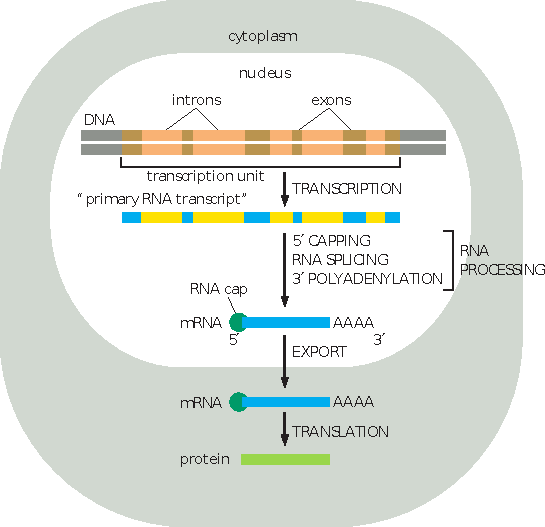
\includegraphics{gene_expression.pdf}
		\caption[Gene expression]{In the cell nucleus, the DNA molecule is transcribed into primary RNAs products. After a step of processing mRNAs are exported from the nucleus to the cytoplasm where the translation of mRNAs into proteins occurs. From~\cite{alberts2022molecular}.}\label{fig:gene_expression}
	\end{figure}

	The DNA molecule, located in the cell nucleus, holds the genetic information of an organism.
	This molecule is transcribed into various RNA products.
	After a maturation step, a pool of these RNAs becomes \glspl{mrna_mol}.
	\glspl{mrna_mol} are exported into the cell cytoplasm, where ribosomes will start the translation of the \gls{mrna_mol} into a protein.
	RNAs producing proteins correspond to coding sequences, or genes,  in the DNA sequence, the non-coding sequences are still transcribed and are involved in regulating gene expression.
	Quantifying all molecular components involved in the correct functioning of a cell generates high-dimensional data.
	Indeed, there are more than 20,000 known coding genes and more than 30,000 known non-coding genes.
	Among the three billion nucleotides in the human genome, 99\% is conserved between individuals.
	The remaining 1\% or thirty million nucleotides are responsible for the phenotypic differences~\cite{GeneticVariation}.

	The data scale highlights the need for computational methods to extract relevant information.
	Machine learning methods have been successfully applied to study omics data and predict phenotypes.
	However, the high dimensionality of omics data is not compatible with current machine learning models without a prior feature selection.
	The selection procedure is decoupled from the prediction task, and only selected features are used for downstream predictions.
	Using only selected features limits the model's capacity to extract hidden information from the omitted features.

	The last decade has witnessed a significant development of deep learning algorithms, which have become a standard in many domains, such as computer vision, speech recognition or natural language processing~\cite{lecunDeepLearning2015}.
	Deep learning can extract and exploit the complete information from all features and their interactions.
	\citeauthor{Hanczar2022}~\cite{Hanczar2022} has shown that with the increasing availability of omics data, deep learning architectures are becoming competitive with the state-of-the-art classical machine learning techniques applied to omics data.
	Various deep learning architectures were successfully applied to omics data.
	While applying deep learning to omics data is successful, it still faces some challenges.
	The high-dimensionality of omics data leads to very large models, \ie{}with many parameters to estimate, making them susceptible to overfitting.
	With classical deep learning models, the weights used to combine features to construct an abstract representation are learned during the training phase.
	During the inference phase, they are fixed and assumed to be identical for all patients.
	However, for a truly personalized medicine, interactions need to be specific for each patient, as cellular functions are governed by the combined action of multiple molecular entities specific to a patient.

	Focusing on individual omics might not be sufficient to capture the full complexity of biological processes.
	Indeed, a mutation in the genome might not correspond to a disease state.
	Due to the degeneracy of the genetic code, a single mutation can have no effect on the final protein form.
	Moreover, gene expression is a highly regulated mechanism.
	The presence of an \gls{mrna_mol} in a cell does not necessarily lead to normal levels of protein synthesis.
	The \gls{mrna_mol} could be targeted by an \gls{mirna}, leading to its degradation, or its half-life could be reduced, limiting its capacity to produce proteins.
	The various molecular actors involved in gene expression regulation show the importance of integrating multi-omics data to improve the predictions made by models.

	Deep learning models can be highly accurate, but they lack transparency on how the predictions were obtained.
	They are referred to as \emph{black-box} models.
	This opacity can significantly limit their adoption in critical applications, such as healthcare,  where understanding the basis of decisions is crucial.
	Interpretability of predictions can help in the adoption of deep learning systems in healthcare as:
	\begin{itemize}[nosep]
		\item it helps the end-user (physician or patient) understand the prediction;
		\item it allows detecting potential biases;
		\item it can be used for knowledge discovery.
	\end{itemize}
	%Enhancing deep learning models with interpretability can help physicians in making informed decisions.

\section{Thesis context and objectives}
	This Ph.D. is a collaboration between the IBISC laboratory\footnote{\url{https://www.ibisc.univ-evry.fr/}} and Sanofi\footnote{\url{https://www.sanofi.com/}} under the \gls{cifre} program.
	The \gls{cifre} program is a French program aiming at strengthening exchanges between academic laboratories and private industries.
	The company receives financial assistance to recruit a doctoral student whose research work is performed under the supervision of the academic partner.
	The program is funded by the French government, and its management is handled by the \gls{anrt}, which approves the collaboration project.

	This collaboration aims to explore the interest of deep learning approaches to integrate and analyze multi-omics data.
	Through this collaboration, Sanofi's goal was to increase its skills in multi-omics data analysis with deep learning methods.
	Sanofi also aims to internalize and apply the developed methods to other internal datasets.
	IBISC laboratory aims to expand its knowledge of multi-omics data by benefiting from Sanofi's expertise and Sanofi's assistance with their expertise in cancer biology to assess potential biomarkers.
	The project proposal defined three main objectives:
	\begin{description}[
			style=multiline,
			leftmargin=!,
			labelwidth=2cm
		]
		\item[First objective]
			Development of a deep learning model for each omics type that limits the risk of overfitting due to the limited size of omics datasets.
			We proposed a novel deep learning for omics type based on the attention mechanism.
			The proposed architecture can incorporate knowledge through the attention mechanism.
		\item[Second objective]
			Development of a predictive model integrating various omics data that can model the dependence of the different omics and be robust to missing modalities during inference.
			We proposed a multi-omics integration method based on cross-attention that effectively considers interactions of pairs of omics known to interact.
			We also established that modality dropout, where one or more modalities are randomly masked during training, is an effective approach to having robust models for different missingness patterns.
		\item[Third objective]
			This objective focused on model interpretation to better understand the studied disease and to identify potential biomarkers.
			We proposed a model integrating multi-omics data with the training objective, forcing the model to focus on the most important interaction.
			The model learns a score for each interaction, and this interaction score provides a first explainability level in understanding how the predictions are obtained.
			We have also proposed a method based on counterfactuals to identify potential biomarkers by finding the minimal realistic change in the prediction.
	\end{description}
	% \clearpage

\section{Thesis overview}
	\begin{center}
		\vspace{-2\baselineskip}
		\ifSubfilesClassLoaded{%
			\begin{spacing}{1}
	\fontsize{10}{10}\selectfont
\begin{tikzpicture}<disable externalization>
	\node[circle, fill=Prune, text=white, draw=Prune] (n1) at (0,0){\ref*{chap:background}};
	\node[circle, fill=Prune, text=white, below=2.5cm of n1.south] (n2) {\ref*{chap:sota}};
	\node[circle, fill=Prune, text=white, below=2.5cm of n2.south] (n3) {\ref*{chap:attomics}};
	\node[circle, fill=Prune, text=white, below=2.5cm of n3.south] (n4) {\ref*{chap:crossattomics}};
	\node[circle, fill=Prune, text=white, below=2.5cm of n4.south] (n5){\ref*{chap:crossattomicsgate}};
	\node[circle, fill=Prune, text=white, below=2.5cm of n5.south] (n6){\ref*{chap:counterfactuals}};

	\draw[Prune, line width=3pt, dashed] (n1.north) -- +(0,1cm);
	\draw[Prune, line width=3pt] (n1.south) -- (n2.north);
	\draw[Prune, line width=3pt] (n2.south) -- (n3.north);
	\draw[Prune, line width=3pt] (n3.south) -- (n4.north);
	\draw[Prune, line width=3pt] (n4.south) -- (n5.north);
	\draw[Prune, line width=3pt] (n5.south) -- (n6.north);
	\draw[Prune, line width=3pt, -{Stealth}] (n6.south) -- +(0,-1cm);

	\tcbset{
		colframe=Prune,
		colback=white,
		colupper=Prune,
		fontupper=\relscale{0.9}\hypersetup{linkcolor=Prune},
		fonttitle=\small\bfseries,
		nobeforeafter,
		tcbox width=auto limited,
		center title,
		width=6cm,
		left=1mm,right=1mm,top=1mm,bottom=1mm, boxsep=1.5mm,
	}

	\node[right=1cm of n1.east, anchor=west] (b1) {
		\tcbox[title=Background]{
			In this chapter, the different deep learning architectures used during this thesis work are presented. A brief presentation of gene expression regulation and cancer formation is done. The methods to obtain the different omics are described. Finally, the different datasets used are described.
		}
	};

	\node[left=1cm of n2.west, anchor=east] (b2) {
		\tcbox[title=State-of-the-art]{
			This chapter is dedicated to the description of the current deep learning methods used to predict a phenotype from omics data. A bried introduction to multimodal machine learning is done before describing its application to integrate multi-omics data.
		}
	}; %4.85 cm available for images

	\node[right=1cm of n3.east, anchor=west] (b3) {
		\tcbox[title=AttOmics]{
			This chapter presents the AttOmics architecture, an architecture based on the attention mechanism. Expression profiles are transformed into groups of features with a transformation \(\symcal{T}\).
			Group are individually projected to compute intra-group interactions.
			\Glsxtrshort{mhsa} is then applied to incorporate inter-group interactions in the representation.
			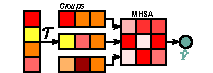
\includegraphics[width=\linewidth]{AttOmics_logo.pdf}
		}
	};

	\node[left=1cm of n4.west, anchor=east] (b4) {
		\tcbox[title=CrossAttOmics]{
			This chapter presents a multiomics extension of the AttOmics architecture. Each omics is encoded with an encoder based on AttOmics. Cross-attention is used to compute interactions between omics with known regulatory links.
			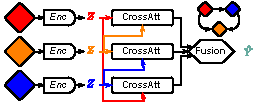
\includegraphics[width=\linewidth]{CrossAttOmics_Logo.pdf}
		}
	};

	\node[right=1cm of n5.east, anchor=west] (b5) {
		\tcbox[title=CrossAttOmicsGate]{
			This chapters present a variation of the CrossAttOmics architecture. Instead of focusing on known omics interactions, cross attention is used on all pairs of omics. Then interactions are scored for each patient.
			This importance score must have enough sparsity to be interpretable and diverse across samples, as omics interactions differ between samples.
		}
	};

	\node[left=1cm of n6.west, anchor=east] (b6) {
		\tcbox[title=Counterfactuals]{
			TEST tesfkl fzlkfes gznjef fe,fbzkf vjnfzefb
		}
	};

	\draw[Prune, line width=1.5pt, -{Circle}] (n1.east) -- (b1.west);
	\draw[Prune, line width=1.5pt, -{Circle}] (n2.west) -- (b2.east);
	\draw[Prune, line width=1.5pt, -{Circle}] (n3.east) -- (b3.west);
	\draw[Prune, line width=1.5pt, -{Circle}] (n4.west) -- (b4.east);
	\draw[Prune, line width=1.5pt, -{Circle}] (n5.east) -- (b5.west);
	\draw[Prune, line width=1.5pt, -{Circle}] (n6.west) -- (b6.east);

	\tcbhypernode{\hyperref[chap:background]}{n1}
	\tcbhypernode{\hyperref[chap:sota]}{n2}
	\tcbhypernode{\hyperref[chap:attomics]}{n3}
	\tcbhypernode{\hyperref[chap:crossattomics]}{n4}
	\tcbhypernode{\hyperref[chap:crossattomicsgate]}{n5}
	\tcbhypernode{\hyperref[chap:counterfactuals]}{n6}

	\tcbhypernode{\hyperref[chap:background]}{b1}
	\tcbhypernode{\hyperref[chap:sota]}{b2}
	\tcbhypernode{\hyperref[chap:attomics]}{b3}
	\tcbhypernode{\hyperref[chap:crossattomics]}{b4}
	\tcbhypernode{\hyperref[chap:crossattomicsgate]}{b5}
	\tcbhypernode{\hyperref[chap:counterfactuals]}{b6}
\end{tikzpicture}
\end{spacing}%
		}{
			\begin{spacing}{1}
	\fontsize{10}{10}\selectfont
\begin{tikzpicture}<disable externalization>
	\node[circle, fill=Prune, text=white, draw=Prune] (n1) at (0,0){\ref*{chap:background}};
	\node[circle, fill=Prune, text=white, below=2.5cm of n1.south] (n2) {\ref*{chap:sota}};
	\node[circle, fill=Prune, text=white, below=2.5cm of n2.south] (n3) {\ref*{chap:attomics}};
	\node[circle, fill=Prune, text=white, below=2.5cm of n3.south] (n4) {\ref*{chap:crossattomics}};
	\node[circle, fill=Prune, text=white, below=2.5cm of n4.south] (n5){\ref*{chap:crossattomicsgate}};
	\node[circle, fill=Prune, text=white, below=2.5cm of n5.south] (n6){\ref*{chap:counterfactuals}};

	\draw[Prune, line width=3pt, dashed] (n1.north) -- +(0,1cm);
	\draw[Prune, line width=3pt] (n1.south) -- (n2.north);
	\draw[Prune, line width=3pt] (n2.south) -- (n3.north);
	\draw[Prune, line width=3pt] (n3.south) -- (n4.north);
	\draw[Prune, line width=3pt] (n4.south) -- (n5.north);
	\draw[Prune, line width=3pt] (n5.south) -- (n6.north);
	\draw[Prune, line width=3pt, -{Stealth}] (n6.south) -- +(0,-1cm);

	\tcbset{
		colframe=Prune,
		colback=white,
		colupper=Prune,
		fontupper=\relscale{0.9}\hypersetup{linkcolor=Prune},
		fonttitle=\small\bfseries,
		nobeforeafter,
		tcbox width=auto limited,
		center title,
		width=6cm,
		left=1mm,right=1mm,top=1mm,bottom=1mm, boxsep=1.5mm,
	}

	\node[right=1cm of n1.east, anchor=west] (b1) {
		\tcbox[title=Background]{
			In this chapter, the different deep learning architectures used during this thesis work are presented. A brief presentation of gene expression regulation and cancer formation is done. The methods to obtain the different omics are described. Finally, the different datasets used are described.
		}
	};

	\node[left=1cm of n2.west, anchor=east] (b2) {
		\tcbox[title=State-of-the-art]{
			This chapter is dedicated to the description of the current deep learning methods used to predict a phenotype from omics data. A bried introduction to multimodal machine learning is done before describing its application to integrate multi-omics data.
		}
	}; %4.85 cm available for images

	\node[right=1cm of n3.east, anchor=west] (b3) {
		\tcbox[title=AttOmics]{
			This chapter presents the AttOmics architecture, an architecture based on the attention mechanism. Expression profiles are transformed into groups of features with a transformation \(\symcal{T}\).
			Group are individually projected to compute intra-group interactions.
			\Glsxtrshort{mhsa} is then applied to incorporate inter-group interactions in the representation.
			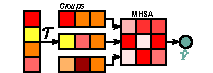
\includegraphics[width=\linewidth]{AttOmics_logo.pdf}
		}
	};

	\node[left=1cm of n4.west, anchor=east] (b4) {
		\tcbox[title=CrossAttOmics]{
			This chapter presents a multiomics extension of the AttOmics architecture. Each omics is encoded with an encoder based on AttOmics. Cross-attention is used to compute interactions between omics with known regulatory links.
			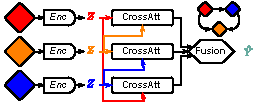
\includegraphics[width=\linewidth]{CrossAttOmics_Logo.pdf}
		}
	};

	\node[right=1cm of n5.east, anchor=west] (b5) {
		\tcbox[title=CrossAttOmicsGate]{
			This chapters present a variation of the CrossAttOmics architecture. Instead of focusing on known omics interactions, cross attention is used on all pairs of omics. Then interactions are scored for each patient.
			This importance score must have enough sparsity to be interpretable and diverse across samples, as omics interactions differ between samples.
		}
	};

	\node[left=1cm of n6.west, anchor=east] (b6) {
		\tcbox[title=Counterfactuals]{
			TEST tesfkl fzlkfes gznjef fe,fbzkf vjnfzefb
		}
	};

	\draw[Prune, line width=1.5pt, -{Circle}] (n1.east) -- (b1.west);
	\draw[Prune, line width=1.5pt, -{Circle}] (n2.west) -- (b2.east);
	\draw[Prune, line width=1.5pt, -{Circle}] (n3.east) -- (b3.west);
	\draw[Prune, line width=1.5pt, -{Circle}] (n4.west) -- (b4.east);
	\draw[Prune, line width=1.5pt, -{Circle}] (n5.east) -- (b5.west);
	\draw[Prune, line width=1.5pt, -{Circle}] (n6.west) -- (b6.east);

	\tcbhypernode{\hyperref[chap:background]}{n1}
	\tcbhypernode{\hyperref[chap:sota]}{n2}
	\tcbhypernode{\hyperref[chap:attomics]}{n3}
	\tcbhypernode{\hyperref[chap:crossattomics]}{n4}
	\tcbhypernode{\hyperref[chap:crossattomicsgate]}{n5}
	\tcbhypernode{\hyperref[chap:counterfactuals]}{n6}

	\tcbhypernode{\hyperref[chap:background]}{b1}
	\tcbhypernode{\hyperref[chap:sota]}{b2}
	\tcbhypernode{\hyperref[chap:attomics]}{b3}
	\tcbhypernode{\hyperref[chap:crossattomics]}{b4}
	\tcbhypernode{\hyperref[chap:crossattomicsgate]}{b5}
	\tcbhypernode{\hyperref[chap:counterfactuals]}{b6}
\end{tikzpicture}
\end{spacing}%
		}
	\end{center}

	%https://arxiv.org/abs/2206.00520
	%https://www.nature.com/articles/s41568-020-00327-9 % Designing deep learning studies in cancer diagnostics
\end{document}
